\documentclass[landscape]{exam}
\usepackage{2in1, lscape} 
\printanswers{}

\printanswers{}

\usepackage{units} 
\usepackage{parskip} 
\usepackage{xfrac} 
\usepackage[fleqn]{amsmath}
\usepackage{commath}
\usepackage{cancel}
\usepackage{float}
\usepackage{mdwlist}
\usepackage{booktabs}
\usepackage{cancel}
\usepackage{polynom}
\usepackage{caption}
\usepackage{fullpage}
\usepackage{comment}
\usepackage{enumerate}
\usepackage{graphicx}
\usepackage{mathtools} 

\everymath{\displaystyle}

\author{}
\date{\today}
\title{Statistics \\ Week Three}

\begin{document}

  \maketitle
  \tableofcontents
  \section{Homework 1}

  Label axes for histogram of old cones. X axis could be either coin age or
  years.

  \section{Roulette}

  \subsection{Overview}

  Each player plays 50 games of roulette placing the same bet each time. Graphs
  are winnings/losses histograms for the players. 

  \subsection{Odd/Even Strategy} % (fold)
  
  \begin{figure}[H]
    \centering
    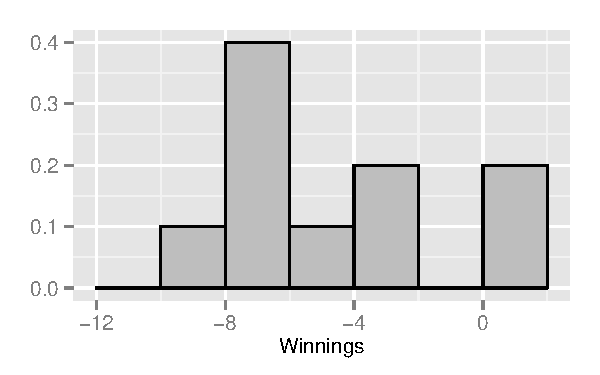
\includegraphics[scale = 0.9]{figures/roulette/18_10_50_fraction.pdf}
    \caption{10 players, odd/even strategy}
  \end{figure}

  \begin{figure}[H]
    \centering
    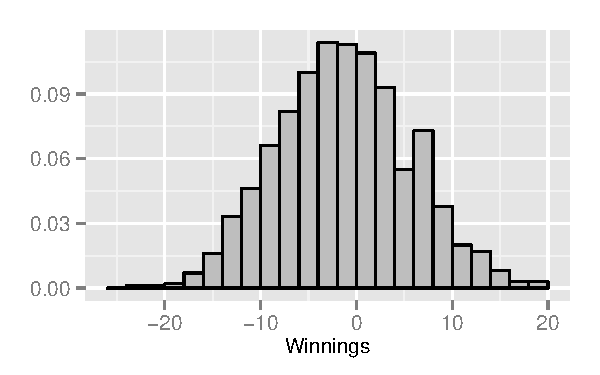
\includegraphics[scale = 0.9]{figures/roulette/18_1000_50_fraction.pdf}
    \caption{1,000 players, odd/even strategy}
  \end{figure}

  \begin{figure}[H]
    \centering
    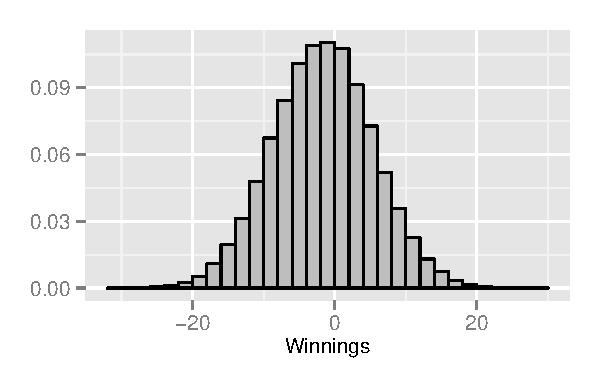
\includegraphics[scale = 0.9]{figures/roulette/18_100000_50_fraction.pdf}
    \caption{100,000 players, odd/even strategy}
  \end{figure}

  \subsection{Four Numbers Strategy} % (fold)
  
  \begin{figure}[H]
    \centering
    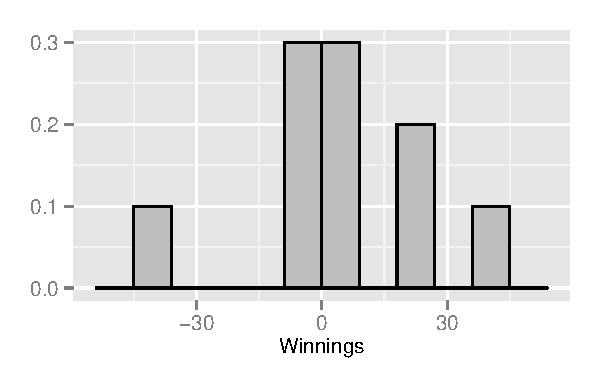
\includegraphics[scale = 0.9]{figures/roulette/4_10_50_fraction.pdf}
    \caption{10 players, four numbers strategy}
  \end{figure}

  \begin{figure}[H]
    \centering
    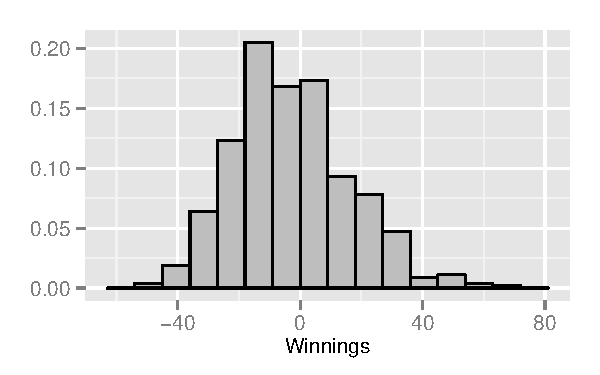
\includegraphics[scale = 0.9]{figures/roulette/4_1000_50_fraction.pdf}
    \caption{1,000 players, four numbers strategy}
  \end{figure}

  \begin{figure}[H]
    \centering
    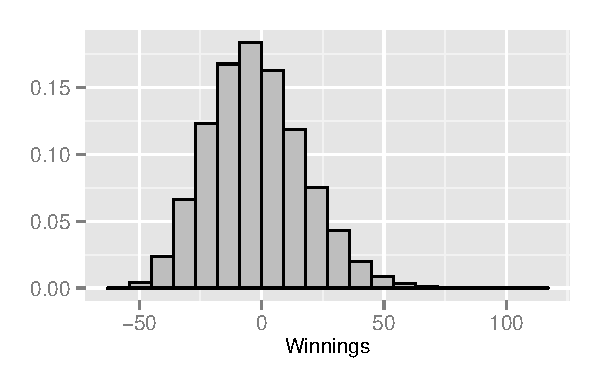
\includegraphics[scale = 0.9]{figures/roulette/4_100000_50_fraction.pdf}
    \caption{100,000 players, four numbers strategy}
  \end{figure}

  \subsection{One Number Strategy} % (fold)
  
  \begin{figure}[H]
    \centering
    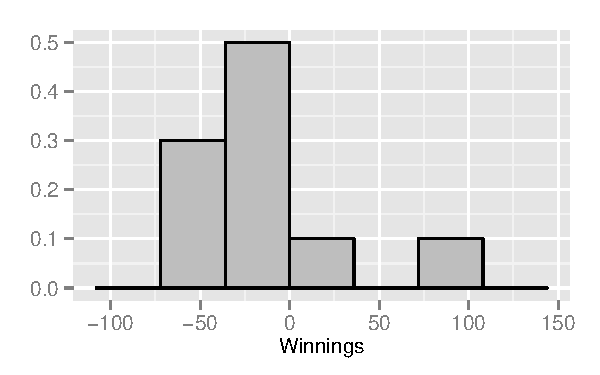
\includegraphics[scale = 0.9]{figures/roulette/1_10_50_fraction.pdf}
    \caption{10 players, one number strategy}
  \end{figure}

  \begin{figure}[H]
    \centering
    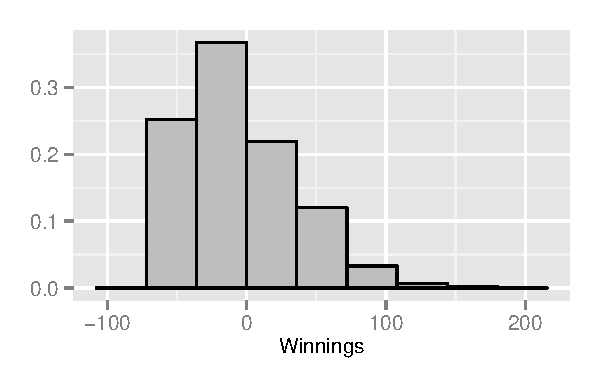
\includegraphics[scale = 0.9]{figures/roulette/1_1000_50_fraction.pdf}
    \caption{1,000 players, one number strategy}
  \end{figure}

  \begin{figure}[H]
    \centering
    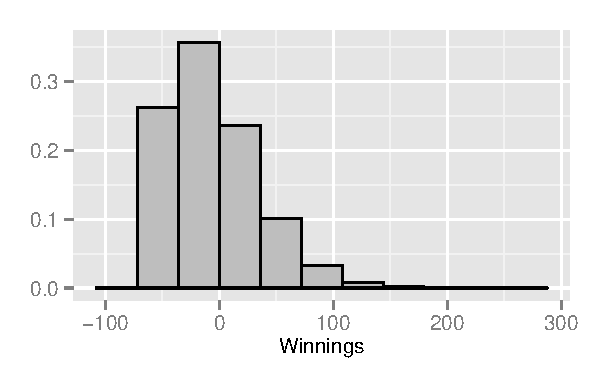
\includegraphics[scale = 0.9]{figures/roulette/1_100000_50_fraction.pdf}
    \caption{100,000 players, one number strategy}
  \end{figure}

  \subsection{Summary} % (fold)
  \begin{table}[H]
    \centering
    \begin{tabular}{lcccc}
      \toprule
      Strategy     & Min   & Max   & Median & $s$ \\
      \midrule
      Odd/Even     & -\$34 & \$26  & -\$2   & \$7.04 \\
      Four Numbers & -\$50 & \$103 & -\$5   & \$19.48 \\
      One Number   & -\$50 & \$274 & -\$14  & \$40.67 \\
      \bottomrule
    \end{tabular}
    \caption{Summary for each strategy, 100,000 players}\label{tab:roulette}
  \end{table}

  \begin{itemize}
    \item With all strategies, mean loss for each player is \$2.64.

    \item Standard deviations, min, max and median are different. 
      See Table~\ref{tab:roulette}.

    \item Second two strategies are right-skewed because there is a limit on how
      much you can lose but essentially no limit on how much you can win. There
      were some players that lost every time with these two strategies.

    \item nobody lost every time with odd/even strategy
  \end{itemize}

  The area under the bars is 1 because
  \begin{align*}
    % A & = \sum_{i = 0}^{100} height \\
    A & = \sum_{i = 0}^{100} \frac{count_i}{totalNumTrials} \\
      & = \frac{\sum_{i = 0}^{100} count_i}{totalNumTrials} \\
      & = \frac{totalNumTrials}{totalNumTrials} \\
      & = 1 \\
  \end{align*}

  If you replace the bars with a smooth curve, the total area under the curve is
  1. This is a probability density curve.

  The curve is approximately a {\em Normal Curve}.  It happens whenever an event
  is either:
  \begin{itemize*}
    \item random chance (coin flip)
    \item complicated combination of factors (test, football play, height, etc.)
    \item central limit theorem
  \end{itemize*}

  Equation for normal curve:
  \[
    f(\mu, \sigma, x) = \frac{1}{\sigma\sqrt{2\pi}} e^{ -\frac{\del{ x-\mu }^2}{2\sigma^2} }
  \]

  $\mu$ is the mean and $\sigma$ is the standard deviation of the
  population. This is different from $\bar{x}$ and $s$ which we use for the mean
  and standard deviation of a sample.

  For any probability distribution:
  \begin{itemize*}
    \item total area under graph is 1

    \item area under curve between $-\infty$ and some x value is probability of
      a value less than that $x$ value.

    \item curve balances at the $\mu$

    \item equal area point is at the median

    \item for a right-skewed curve, mean is to the right of the median. Opposite
      for left-skewed curve.
  \end{itemize*}

  For a Normal curve:
  \begin{itemize*}
    \item 68\% of the values are within one standard deviation of the mean.

    \item 95\% of the values are within two standard deviations of the mean.

    \item 99.7\% of the values are within three standard deviations of the mean.

    \item graph changes curvature at $\mu \pm \sigma$.

  \end{itemize*}

  Get normal curves from computer or table in back of the book.

  Standard normal distribution is normal distribution with $\mu = 0$ and
  $\sigma = 1$.

  \section{Z-score}

  How to you know how likely a particular outcome is?  All the graphs have
  different ranges on the x and y axes.
  
  Convert every score to a z-score. A z-score indicates how far from the mean a
  score is in standard deviation units.

  Formula for z score is:
  \[
    z = \frac{x - \mu}{\sigma}
  \]

  Units for z-scores are standard deviations.

  If original score is $N(\mu, \sigma)$, z-scores have a standard Normal
  ($N(0, 1)$) distribution. 

  \begin{table}
    \centering
    \begin{tabular}[H]{rrrr}
      \toprule
      Outcome & Odd/Even & Four Numbers & One Number \\
      \midrule
      \$-50   & -6.7714  & -2.4308      & -1.1646 \\
      \$-20   & -2.4857  & -0.8923      & -0.4275 \\
      \$-10   & -1.0571  & -0.3795      & -0.1818 \\
      \$0     & 0.3714   & 0.1333       & 0.0639  \\
      \$10    & 1.8      & 0.6462       & 0.3096 \\
      \$20    & 3.2286   & 1.159        & 0.5553 \\
      \$50    & 7.5143   & 2.6974       & 1.2924 \\
      \bottomrule
    \end{tabular}
    \caption{z-scores}\label{tab:z-scores}
  \end{table}

  \begin{table}
    \centering
    \begin{tabular}[H]{rrrr}
      \toprule
      Outcome & Odd/Even & Four Numbers & One Number \\
      \midrule
      \$-50   & 0.00     & 0.01         & 0.12 \\
      \$-20   & 0.01     & 0.19         & 0.33 \\
      \$-10   & 0.15     & 0.35         & 0.43 \\
      \$0     & 0.36     & 0.45         & 0.47  \\
      \$10    & 0.96     & 0.74         & 0.62 \\
      \$20    & 1.00     & 0.88         & 0.71 \\
      \$50    & 1.00     & 1.00         & 0.90 \\
      \bottomrule
    \end{tabular}
    \caption{Chance of winning less than Outcome. Some numbers differ
    from book table.}\label{tab:percentages}
  \end{table}

  You can go from a percentile to a z-score using the table in the back of the
  book.

  You can go from z-score to x by solving for x:
  \begin{align*}
    z &= \frac{x - \mu}{\sigma} \\
    x &= z \sigma + \mu \\
  \end{align*}

  \begin{table}
    \centering
    \begin{tabular}[H]{rrrrr}
      \toprule
      Quantile & z-score & Odd/Even & Four Numbers & One Number \\
      \midrule
      0.1 \    & -1.2815 & -\$11.57 & -\$27.59     & -\$54.76 \\
      0.25 \   & -0.6745 & -\$7.32  & -\$15.75     & -\$30.05 \\
      0.5 \    & 0       & -\$2.60  & -\$2.60      & -\$2.60 \\
      0.75 \   & 0.6745  & \$2.12   & \$10.55      & \$24.85 \\
      0.90 \   & 1.2815  & \$6.37   & \$11.39      & \$49.56 \\
      \bottomrule
    \end{tabular}
    \caption{Result by percentile}\label{tab:quantiles}
  \end{table}
  
  You can subtract to get ranges. For example, 80\% of the people will be
  somewhere between losing \$11.57 and winning \$6.37 when using the odd/even
  strategy.

  \begin{itemize*}
    \item Table in back of book has more precision and different row/column
      arrangement to save space.
    \item table is ``what fraction is less than x'' and not ``what fraction is
      exactly x''.  With continuous things like height and weight, no fraction is
      exactly any particular value.
  \end{itemize*}

  \section{NFL}

  \begin{figure}[H]
    \centering
    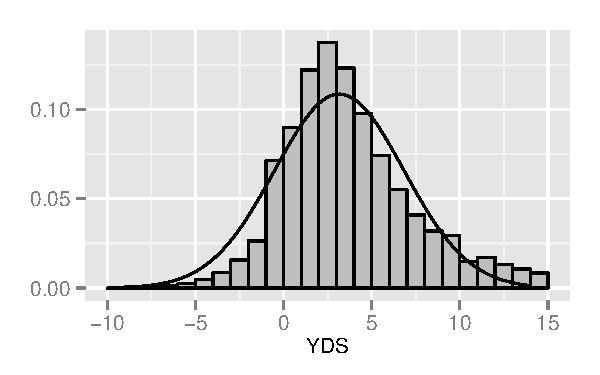
\includegraphics[scale = 0.9]{figures/nfl/yards_per_rush.pdf}
    \caption{Yards per rush, removing outliers}
  \end{figure}

  \begin{align*}
    \mu    & \approx \unit[3.2]{yd} \\
    \sigma & \approx \unit[3.7]{yd} \\
  \end{align*}

  \begin{questions}
    \question{} What percentage of rushes are less than 5 yards?
      \begin{solution}
        \begin{align*}
          z & = \frac{5 - 3.2}{3.7} \\
            & \approx 0.4865 \\
        \end{align*}

        From table in back of book, $p \approx 0.6867$.
      \end{solution}

    \question{} What percentage of rushes are losses?
      \begin{solution}
        \begin{align*}
          z & = \frac{0 - 3.2}{3.7} \\
            & \approx 0.-0.8648 \\
        \end{align*}

        From table in back of book, $p \approx 0.1922$.
      \end{solution}

  \end{questions}

  \section{Students}
  \begin{figure}[H]
    \centering
    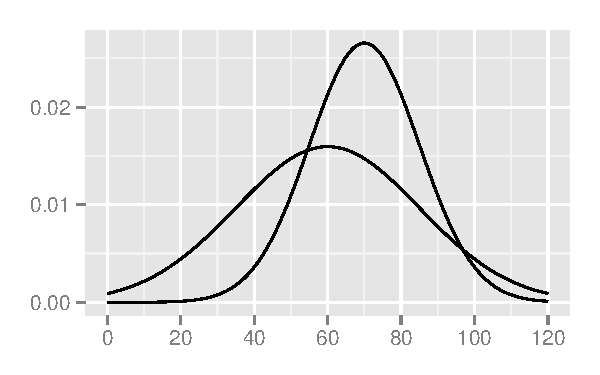
\includegraphics[scale = 0.9]{figures/two_tests.pdf}
    \caption{Two tests}
  \end{figure}

  \begin{itemize*}
    \item $\mu = 70$ and $\sigma = 15$
    \item $\mu = 60$ and $\sigma = 25$
  \end{itemize*}

  \begin{itemize*}
    \item What does a score of 50 mean in each test?
      \begin{solution}
        \begin{itemize*}
          \item 34th percentile on 60 mean test
          \item 9th percentile on 75 mean test
        \end{itemize*}
      \end{solution}

    \item What does a score of 85 mean in each test?
      \begin{solution}
        84th percentile in both tests.  85 is one standard deviation above the
        mean in both cases.
      \end{solution}

    \item What score do you need for 95th percentile in each test?
      \begin{solution}
        \begin{itemize*}
          \item 101 on 60 mean test
          \item 95 on 75 mean test
        \end{itemize*}
      \end{solution}

  \end{itemize*}

  \section{Apply Your Knowledge} % (fold)

  \begin{description}
    \item[3.5]
      See Figure~\ref{fig:ayn_3.5}

      \begin{figure}[H]
        \centering
        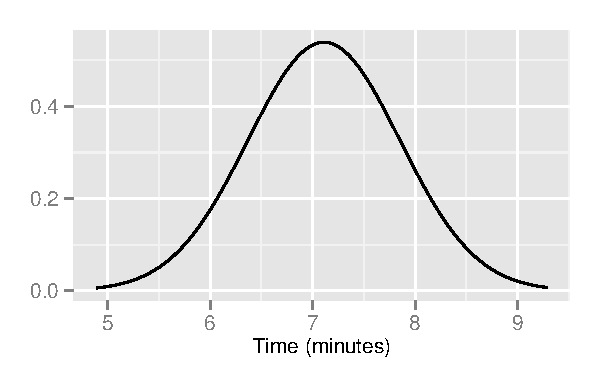
\includegraphics[scale = 0.9]{figures/ayn_3_5.pdf}
        \caption{Apply Your Knowledge 3.5}\label{fig:ayn_3.5}
      \end{figure}

    \item[3.6]
      \begin{enumerate}[(a)]
        \item 4.89 to 9.33 minutes

        \item $1 - (.5 + .34) = 0.16$
      \end{enumerate}

    \item[3.7]
      \begin{enumerate}[(a)]
        \item 688 to 1016 millimeters

        \item less than 688 millimeters
      \end{enumerate}

    \item[3.8] Eleanor's z-score is 1.447. Gerald's z-score is 1.176. Elanor did
      better.

    \item[3.9] The z-score for a 6 foot man is 0.9643. The z-score for a 6 foot
      woman is 2.96. 6-foot tall women are rare. 6-foot tall men are pretty
      common.

    \item[3.11]
      \begin{enumerate}[(a)]
        \item approximately 2%\%
        \item approximately 96\%
      \end{enumerate}

    \item[3.12]
      \begin{enumerate}[(a)]
        \item 90\%
        \item 9.5\%
      \end{enumerate}

    \item[3.14]
      \begin{enumerate}[(a)]
        \item 0.75, 0.8, 0.85
      \end{enumerate}
  \end{description}
  
\end{document}

